
\subsection{Temperatur}\label{sec:temperatur}
Logiken för avläsning av temperatur är uppdelad i ett antal delblock. Dels för att vara lättöverskådligt, men även så att man lätt ska kunna lägga till funktionalitet i efterhand. Slutanvändaren använder endast \nameref{sec:ds18s20} direkt. Onewire modulen är inte bunden till just DS12S20, utan kan även användas till andra andra enheter som använder sig utav 1-wire protokollet.

All logik använder sig utav VHDL-standardbiblioteket \signal{numeric\_std} för hantering av tal med och utan tecken.

%%% DS18S20 %%%%%%%%%%%%%%%%%%%%%%%%%%%%%%%%%%%%%%%%%%%%%%%%%%%%%%%%%
\subsubsection{DS18S20}\label{sec:ds18s20}
\paragraph{Interface}
DS18S20 exponerar ett interface för mätning och avläsning av nuvarande temperatur. Mätningen initieras genom att \signal{measure} sätts till \signal{'1'}. När temperaturmätningen är klar kommer \signal{valid} sättas till \signal{'1'}.
Då finns temperaturen att avläsa på \signal{temperature} som ett binärt 8 bitars tal på tvåkomplementsform där där bit 7--1 är heltalsdelen och bit 0 decimaldelen.
\signal{valid} fortsätter att vara \signal{'1'} tills en ny mätning initieras genom att \signal{measure} återigen sätts till \signal{'1'}.

En temperaturmätning tar upp till 750ms.
\begin{figure}[htp]
\centering
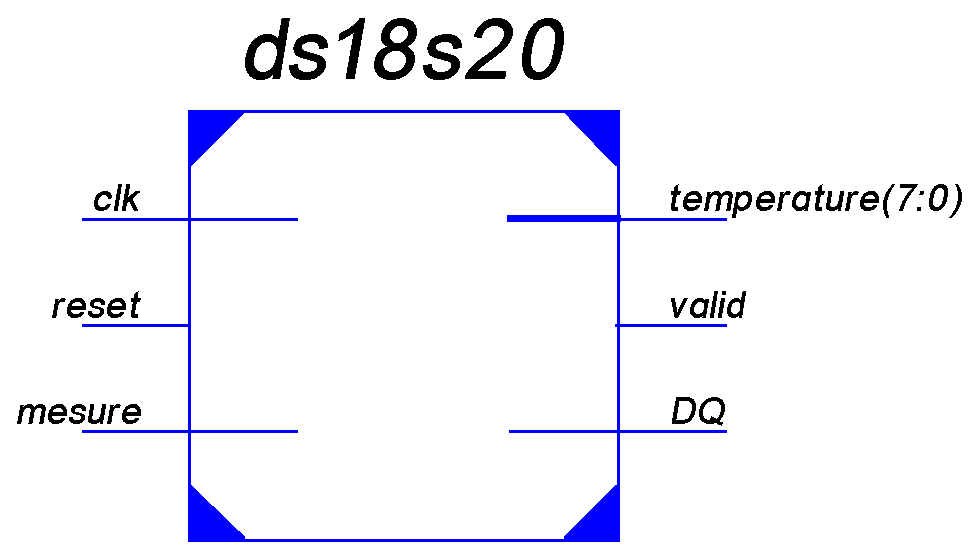
\includegraphics[scale=0.5]{ds18s20_sch.eps}
\caption{Delblocket DS18S20}
\end{figure}

\paragraph{Implementation}
Själva logiken i sig består av en cirkulär tillståndsmaskin (\autoref{fig:ds18s20_fsm}).
Tillståndsmaskinen växlar mellan att ge olika kommandon till onewire-blocket, och sedan vänta på att kommandot ska utföras. En mer utförlig beskrivning när data avläses och hur det samplas finns under \ref{sec:onewire} \nameref{sec:onewire}.
DS18S20 har stöd för flera sensorer på samma buss. De delar då DQ och varje sensor har unikt serienummer för identifiering. I denna konstruktion används endast en sensor och logik för identifiering av flera sensorer utelämnas.

VHDL koden är uppbyggd efter tvåprocessmodellen, med en klockad och en kombinatorisk process.


\begin{table}[H]

\begin{tabularx}{\textwidth}[h]{c c X}
	\hline
	\textbf{Master} & \textbf{Data} & \textbf{Kommentar} \\
	\hline
	
	\Tx & Reset & Reset puls.\\
	\Rx & Presence & Sensorn svarar med en presence puls.\\
	\Tx & 0x44 & Skip ROM command. Eftersom det bara finns en sensor på bussen skippas identifiering.\\
	\Tx & 0x44 & Convert T command. Sensorn mäter och sparar nuvarande temperatur till sitt interna minne.\\
	\Rx & & Sensorn pollas kontinuerligt tills den svarar \high{}, vilket indikerar att mätningen är klar.\\
	\Tx & Reset & Reset puls.\\
	\Rx & Presence & Sensorn svarar med en presence puls.\\
	\Tx & 0x44 & Skip ROM command. Eftersom det bara finns en sensor på bussen skippas identifiering.\\
	\Tx & 0xBE & Read scratchpad command. Läser sensorns interna minne.  \\
	\Rx & <1 byte> & Läser första byten vilket är temperaturen.\\
	
	\hline
\end{tabularx}
\caption{Kontrollsekvens för mätning och avläsning av temperatur}
\end{table}


\begin{figure}[H]
	\centering
	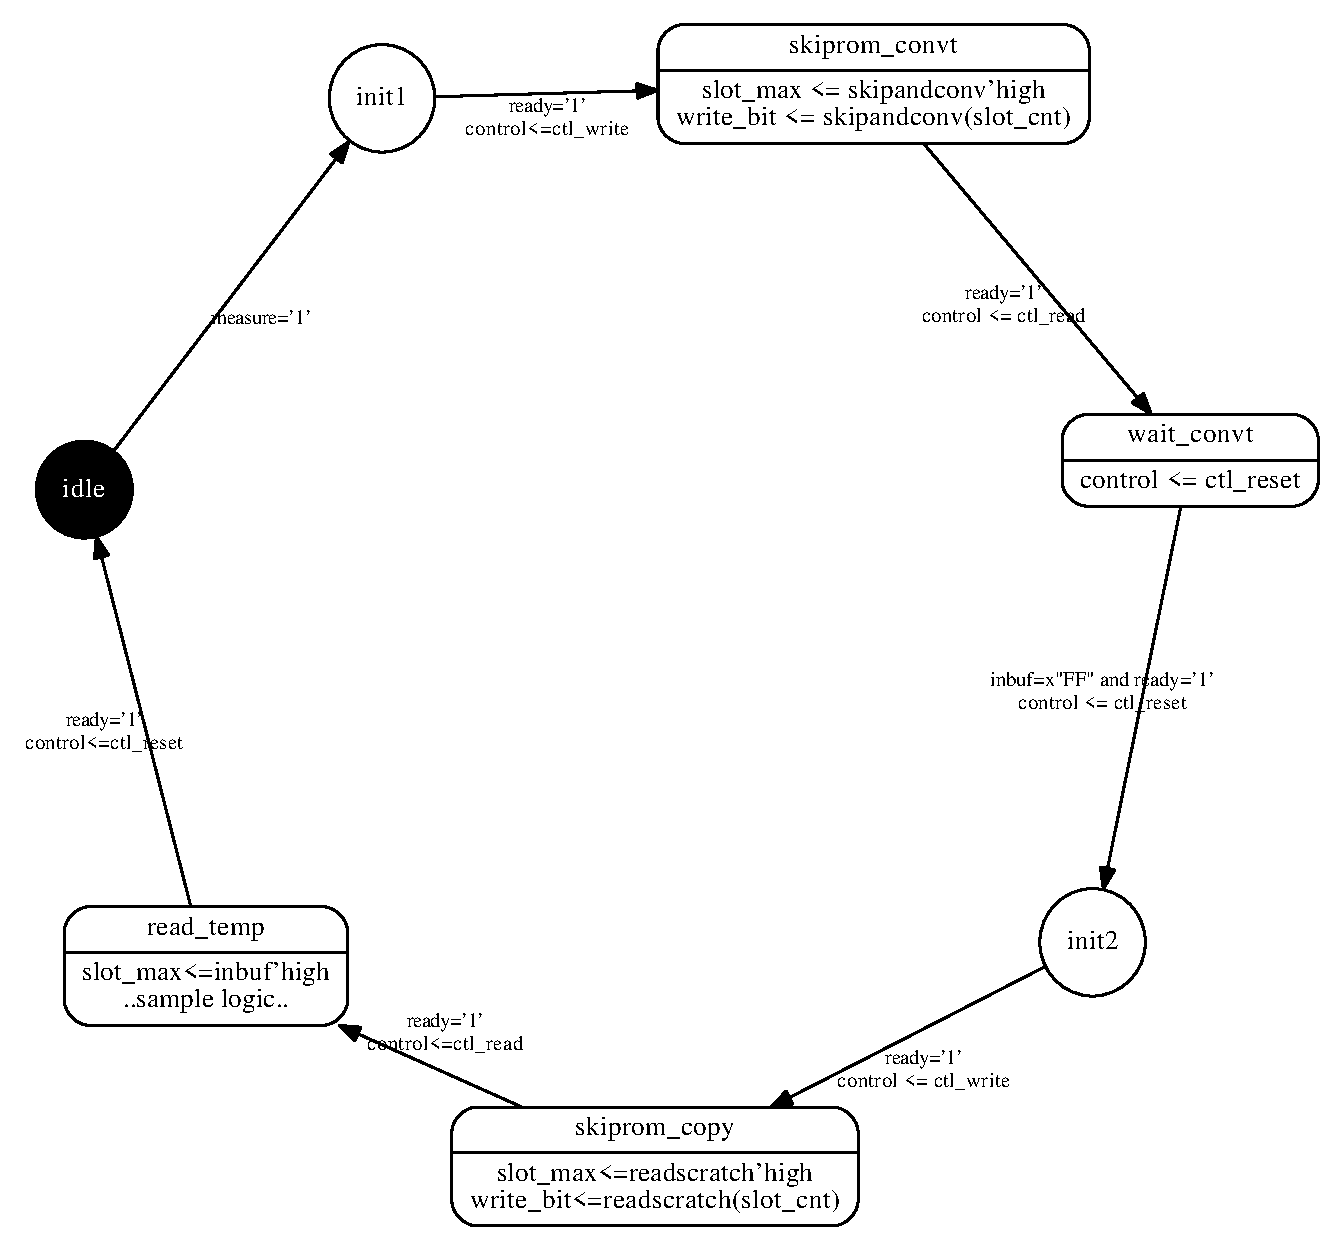
\includegraphics[width=\textwidth]{ds18s20_fsm.eps}
	\caption{Tillståndsmaskin för delblocket DS18S20}
	\label{fig:ds18s20_fsm}
\end{figure}



\subsubsection{Onewire}\label{sec:onewire}
\paragraph{Interface}
Delblocket onwire sköter lågnivå kommunikationen med temperatursensorn, och exponerar ett högre nivå interface med fyra kontroll-kommandon och en ready signal. För att initiera en operation sätts \signal{control} signalen till ett av följande värden när \signal{ready='1'}:

\begin{description}
\item[ctl\_idle] Gör ingenting. \signal{ready} kommer konstant vara \signal{'1'}.

\item[ctl\_read] Läs \signal{slot\_max} antal bitar från sensorn. \signal{slot\_cnt} är en räknare som indikerar vilken bit som läses just nu. När \signal{sample\_now='1'} Förväntas användaren spara biten som under den klockcykeln finns på \signal{read\_bit}. När alla bitar är lästa kommer \signal{ready} sättas till \signal{'1'}.

\textbf{Exempel:}
\begin{lstlisting}
if rising_edge(clk) then
	if sample_now = '1' then
		in_buffer(slot_cnt) <= read_bit;
	end if;
end if;
\end{lstlisting}


\item[ctl\_write] Skriv \signal{slot\_max} antal bitar till sensorn. \signal{slot\_cnt} är en räknare som indikerar vilken bit som skrivs just nu. Användaren förväntas lägga biten som ska skrivas till sensorn på \signal{write\_bit}.
När alla bitar är skrivna kommer \signal{ready} sättas till \signal{'1'}.

\textbf{Exempel:}
\begin{lstlisting}
write_bit <= out_buffer(slot_cnt);
\end{lstlisting}

\item[ctl\_reset] Återställer sensorns tillståndsmaskin.
När reset-sekvensen är klar kommer \signal{ready} sättas till \signal{'1'}.


\end{description}
Under en pågående operation kommer \signal{ready} vara \signal{'0'}.
Observera att efter ``power on'' eller ``master reset'' kommer onewire utföra reset-sekvensen för sensorn, och användaren måste vänta på \signal{ready='1'} innan ett kontrollkommando kan ges.
Det finns även en \signal{error} signal som kommer gå hög under en klockcykel om inte temperatursensorn svarar under resetsekvensen.
\begin{figure}[H]
	\centering
	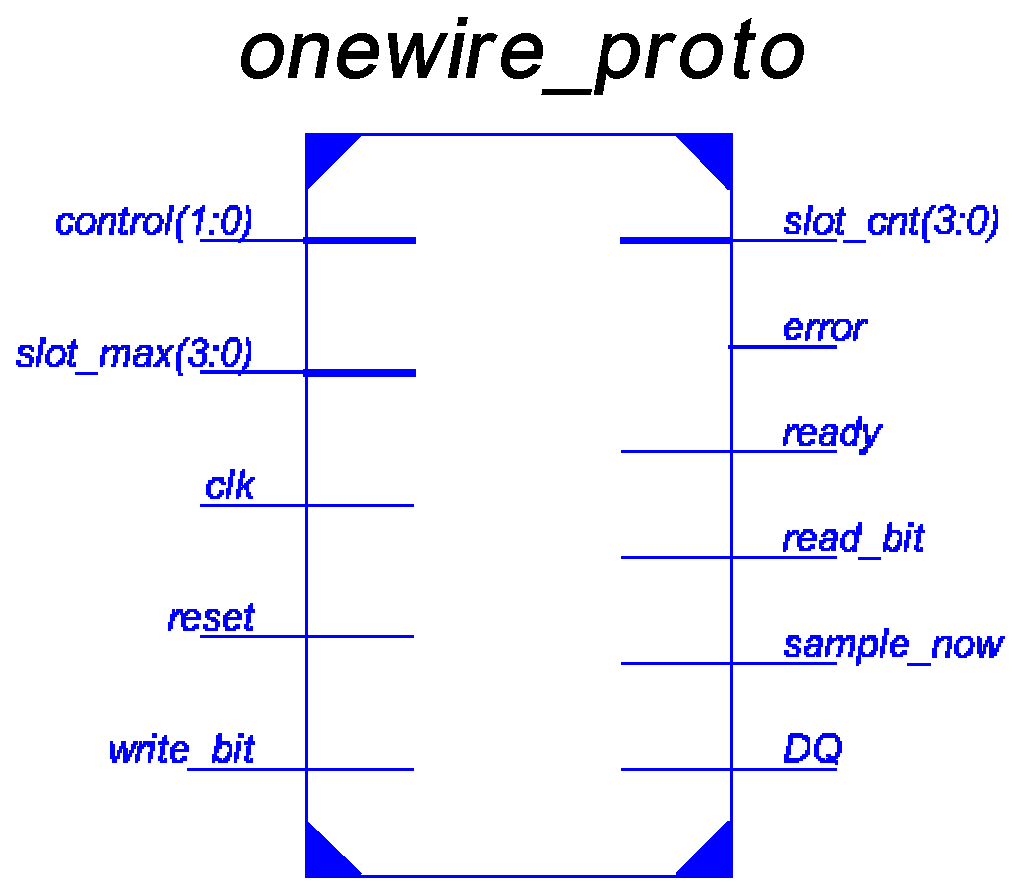
\includegraphics[scale=0.5]{onewire_sch.eps}
	\caption{Delblocket onewire}
\end{figure}

\paragraph{Implementation}
Onewire delblocket implementerar Dallas 1-wire protokoll. För 1-wire används enbart en pin (DQ) för kommunikation. Ingen gemensam klocka finns. 1-wire bygger på master-slave principen, med sensorn som slave och kontrollen som master. Till DQ är en 5K\ohm pullup resistor kopplad. Kommunikation sker via \emph{write slots} och \emph{read slots}. Mastern initierar all kommunikation. 1-wire är \emph{open drain}, vilket innebär att pullup resistorn driver DQ hög när det inte är någon aktivitet på bussen. All data skrivs och avläses med den minst signifikanta biten först (LSB).

1-wire har stöd för sk. ``parasite power'', där DQ driver temperatursensorn. Onewire delblocket använder sig dock inte utav denna funktion, utan sensorn drivs genom $V_{dd}$.

Kontrollen är uppbyggd av en tillståndsmaskin, se \autoref{fig:onewire_fsm}. VHDL koden är uppbyggd efter tvåprocessmodellen, med en klockad och en kombinatorisk process.

\begin{figure}[H]
\centering
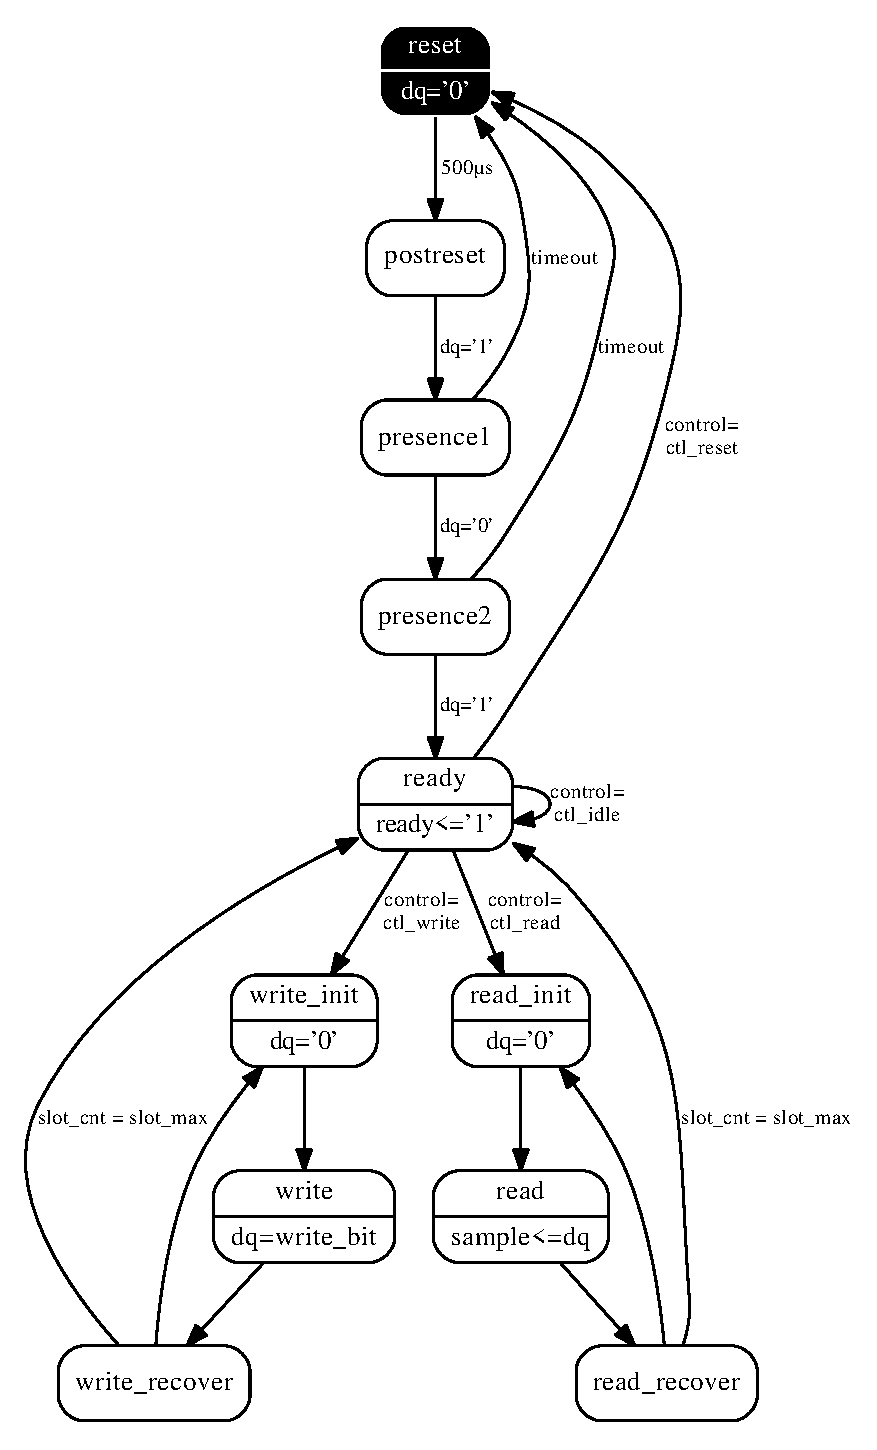
\includegraphics[height=0.97\textheight]{onewire_fsm.eps}
\caption{Tillståndsmaskin för delblocket onewire}
\label{fig:onewire_fsm}
\end{figure}


\subparagraph{Reset}
Resetfasen korresponderar till $reset\rightarrow postreset\rightarrow presence1\rightarrow presence2\rightarrow ready$ i onewires tillståndsmaskin (\autoref{fig:onewire_fsm}).

Vid FPGAns \emph{power on}, eller när den globala, asynkrona \signal{reset} signalen går från hög till låg kommer tillståndsmaskinen börja i \state{reset}. Initieringssekvensen för temperatursensorn DS18S20 kommer då inledas. Se \autoref{fig:ow_timings}. Om temperatursensorn svarar med en korrekt \emph{presence pulse} inom accepterade tidsintervall kommer onewire att försättas i tillstånd \state{ready} och invänta vidare kommandon. Vid felaktigt eller uteblivet svar kommer \signal{error} vara \high{} under en klockcykel. Tillståndsmaskinen kommer sedan återgå till \state{reset} och börja om initieringssekvensen.

\begin{figure}[H]
	\centering
	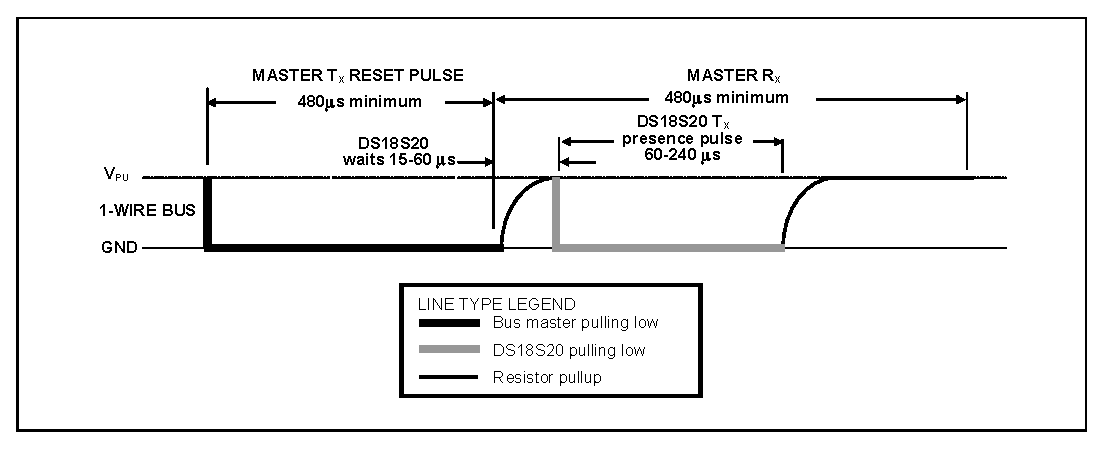
\includegraphics[width=\textwidth]{reset_presence.eps}
	\caption{Tidsspecifikation för 1-wire resetsekvens}
	\label{fig:ow_timings}
\end{figure}


\subparagraph{Skrivning med \emph{write slots}}
Skrivfasen korresponderar till $ready\rightarrow write\_init\rightarrow write\rightarrow write\_recover$ i onewires tillståndsmaskin (\autoref{fig:onewire_fsm}).

För att påbörja en skrivning sätts \signal{control} till \signal{ctl\_write} när \signal{ready='1'}.
\signal{slot\_max} bitar kommer då skrivas till sensorn.
1-wire protokollet använder \emph{write slots} för att skriva bitar till sensorn. Flera bitar skrivs genom flera efterföljande write slots.

En write slot börjar med att buss-mastern driver DQ låg 1--15\us. Sensorn kommer sampla värdet på bussen 15--60\us efter att DQ gick från hög till låg. Efter varje write slot behövs >1\us återhämtningstid.

För att skriva \low{} driver kontrollen DQ låg i 60\us{} < \Tx{} < 120\us{}.
För att skriva \high{} släpper kontrollen DQ maximalt 15\us{} efter att write slot påbörjades.
Se \autoref{fig:rwslots}.


\subparagraph{Läsning med \emph{read slots}}
Läsfasen korresponderar till $ready\rightarrow read\_init\rightarrow read\rightarrow read\_recover$ i onewires tillståndsmaskin (\autoref{fig:onewire_fsm}).

För att påbörja en läsning sätts \signal{control} till \signal{ctl\_read} när \signal{ready='1'}.
\signal{slot\_max} bitar kommer då läsas från sensorn.
1-wire protokollet använder \emph{read slots} för att skriva bitar till sensorn. Flera bitar skrivs genom flera efterföljande read slots.
En read slot initieras alltid av mastern genom att driva DQ låg i 1\us{} < \Tx{} < 15\us{}. Sensorn kommer efter att DQ gått från \high{} $\rightarrow$ \low{} lägga ut \high{} eller \low{} på DQ. Data är giltig upp till 15\us{} efter det att master initierar read slot.
Se \autoref{fig:rwslots}.



\begin{figure}
\centering
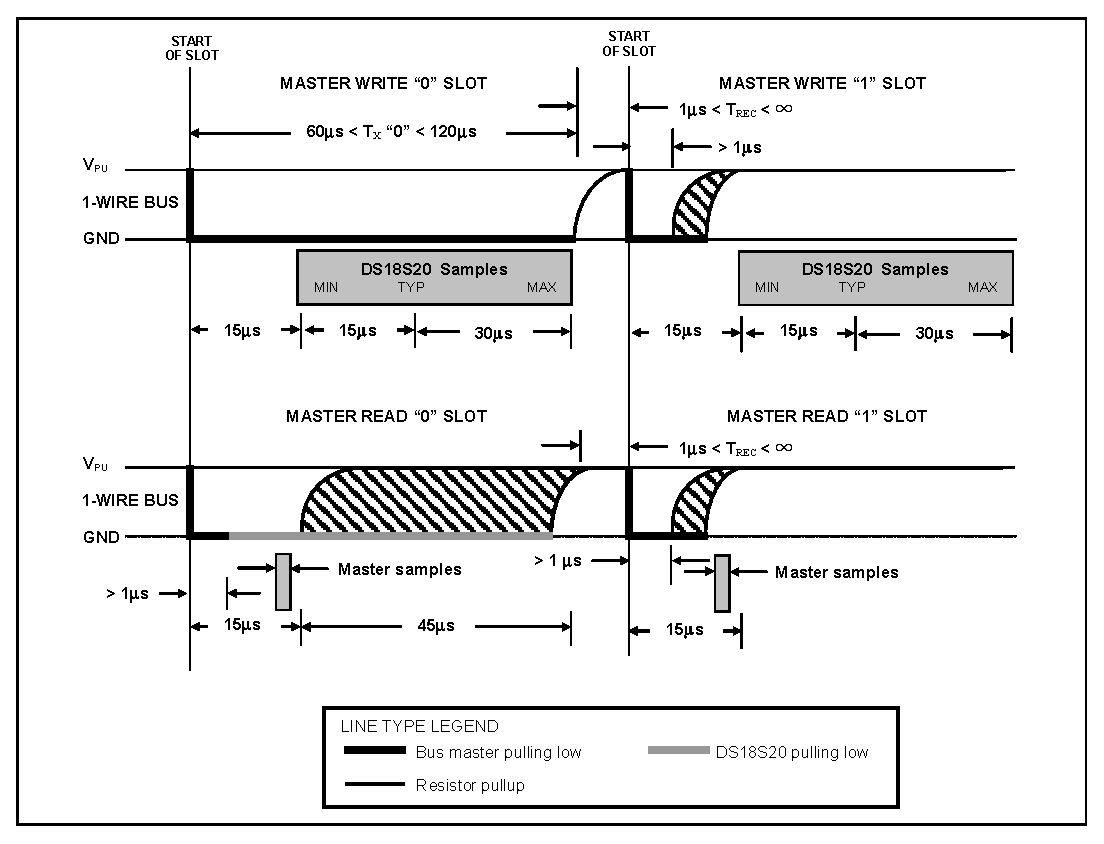
\includegraphics[width=\textwidth]{write_slot.eps}
\caption{Write och read slots tidsspecifikation för \low{} respektive \high{}.}
\label{fig:rwslots}
\end{figure}



%%% 7-segmentsdisplay %%%%%%%%%%%%%%%%%%%%%%%%%%%%%%%%%%%%%%%%%%%%%%%%%%%%%%%%%%%
\subsection{7-Segmentdisplay}\label{sec:7seg}
Delblocket ansvarar för att visa ett 8 bitars binärt tal på tvåkomplementsform där bit 7--1 är heltalsdelen och bit 0 decimaldelen på en 7-segmentdisplay med basen 10.

Det finns stöd för att visa tal mellan -99 -- 999, med en decimalsiffra som antingen är .0 eller .5. Det är tillräckligt för temperatursensorn som är specifierad mellan $-75 -- 125 \pm5$.
\subsubsection{segment-temperature}

\paragraph{Interface}
Komponenten tar ett binärt tal som input och ger utsignalerna till 7-segmentdisplayerna.

<bild>

\paragraph{Implementation}
De fyra fysiska 7-segmentdisplayerna har en gemensam databuss. Varje display har även en enable signal. Komponenten växlar mellan att visa de olika displayerna med 1kHz, vilket för ögat upplevs som att alla lyser konstant.
\paragraph{bcd}\label{sec:bcd}
Funktion som gör om ett binärt tal utan tecken till bcd-form. ``Double Dabble'' algoritmen används internt i form utav ett kombinatoriskt nät.


\begin{figure}[htp]
\centering
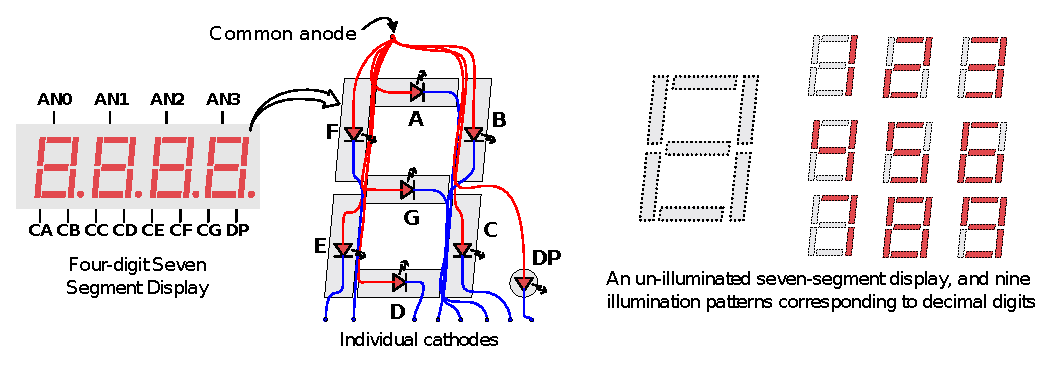
\includegraphics[width=\textwidth]{segment.eps}
\caption{7-segments display}
\label{}
\end{figure}